\documentclass[]{auvsi_doc}
\setkeys{auvsi_doc.cls}{
	AUVSITitle={Imaging Requirements Matrix},
	AUVSILogoPath={./../../../../_resources_/logo.pdf}
}

% include extra packages, if needed
\usepackage{graphicx}

\begin{document}

\begin{AUVSITitlePage}
\begin{artifacttable}
	\entry{IM-007, 1.0, 02-20-19, Measured and predicted values, Tyler Miller \& Jake Johnson, Connor Olsen}
% additional \entry{} commands for extra rows in the revision table, if needed
\end{artifacttable}
\end{AUVSITitlePage}

% document contents (see below for LaTex commands that make your life easier)
\section{Introduction}
Figure \ref{fig:imgReq} shows our updated requirements matrix for the imaging 
subsystem. Predicted and measured values, as well as market response were added 
where applicable. Some values can not be fully measured until multiple flight tests
are performed with imaging fully integrated into the plane.

\begin{figure}[h!]
	%\centering
	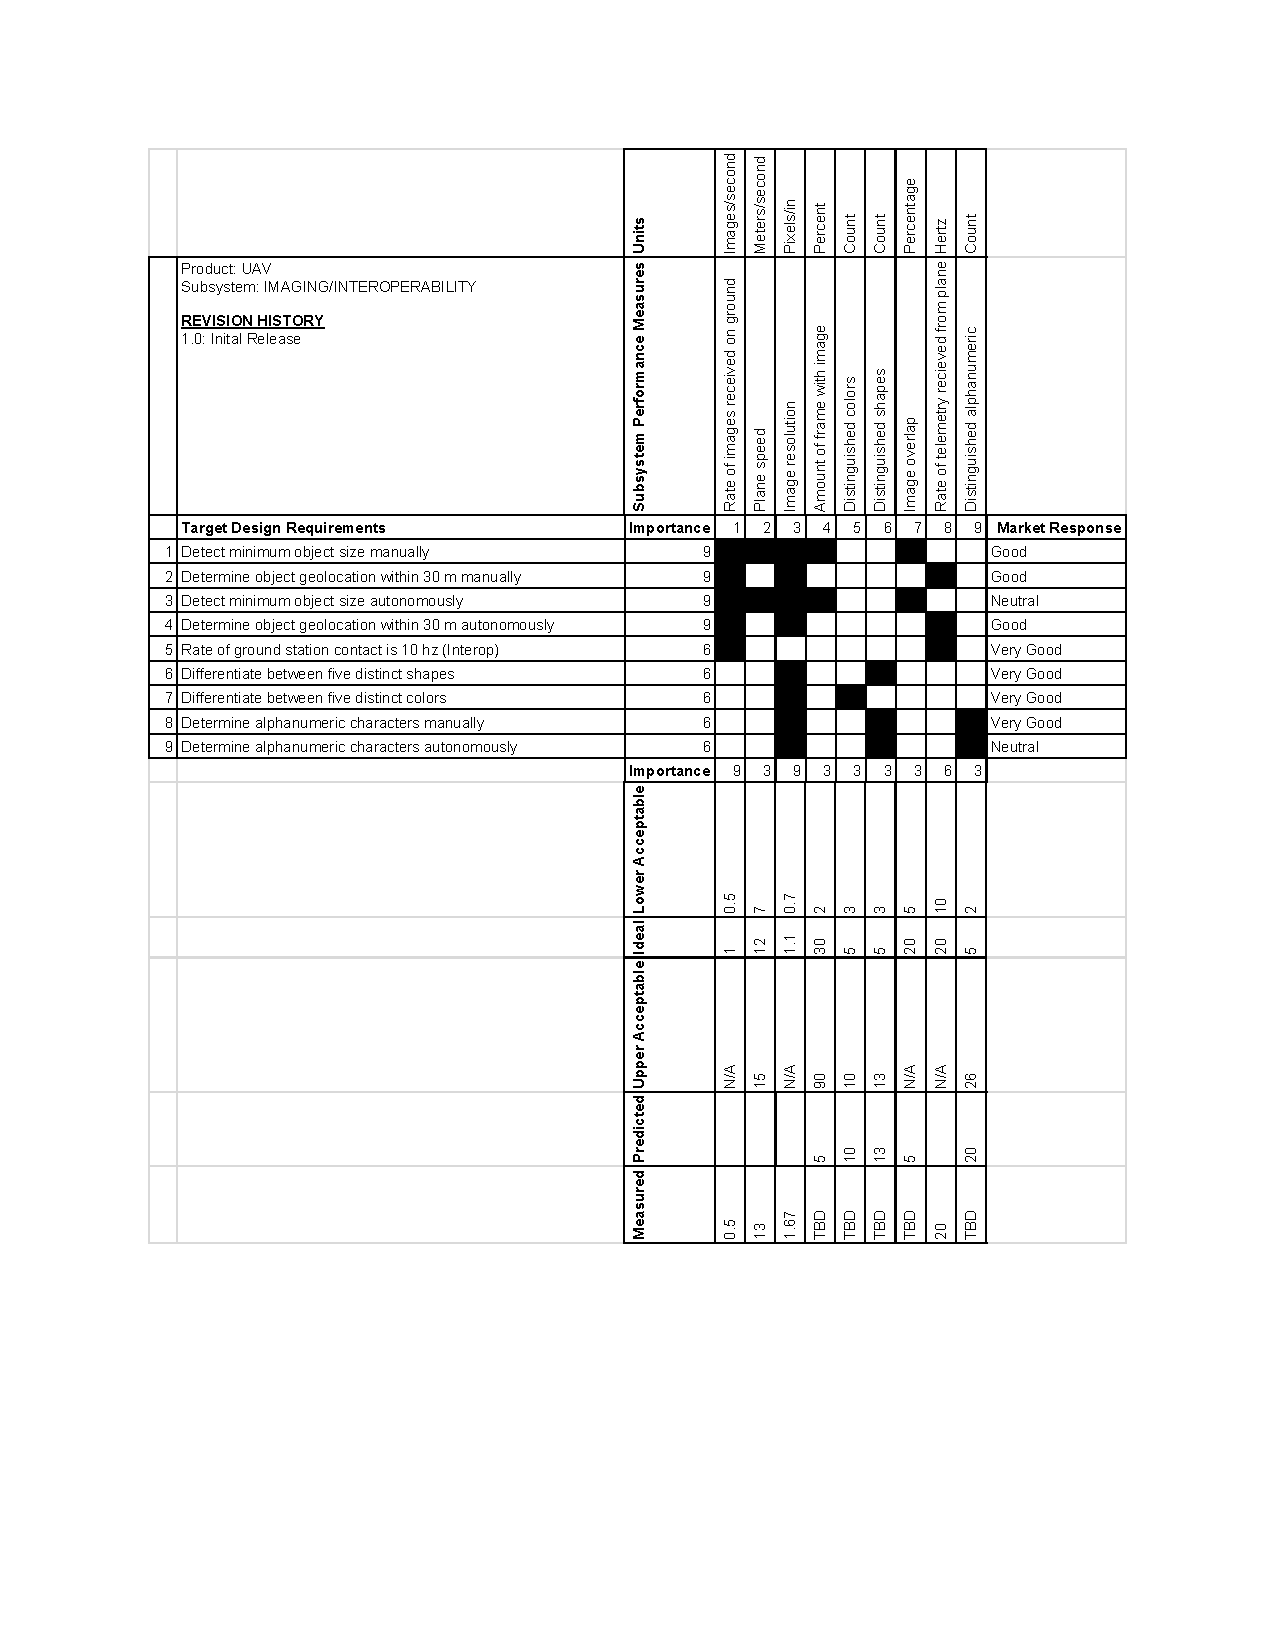
\includegraphics[width=1.2\columnwidth]{./figs/imgReqMatrix.pdf}
	\caption{The updated requirements matrix for the airframe subsystem, with section E included (target, predicted and measured values for performance measures.)}
	\label{fig:imgReq}
\end{figure}

\end{document}
